\section{Introduction}

In genomic analysis, to assess whether
there is an enrichment of one set of features near another 
one must choose an appropriate null model \citep{reviewdilemma2014}.
% -- better save this for later...
%or a correlation across samples between nearby genomic features of
%different modalities (e.g. gene expression, chromatin accessibility).
For example, an enrichment of ATAC-seq peaks near certain genes
may indicate a regulatory relationship \citep{lee2020fluent},
and enrichment of GWAS SNPs near tissue-specific ATAC-seq peaks may
suggest mechanisms underlying the GWAS trait.
Such analyses rely on specifying a null distribution, where one
strategy is to uniformly shuffle one set of the
genomic features in the genome, possibly while considering a set of
excluded regions.
%giving random positions drawn uniformly along the
%genome to existing features, possibly while considering a set of
%excluded positions.
However, uniformly distributed null feature sets will not exhibit the
spatial clumping common with genomic feature sets.
% where there often exists a complex dependency structure.
% both in terms of placement and
% correlation of metadata (signal strength, cell-type-specificity, etc.).
Using an overly simplistic null distribution that doesn't take into
account local dependencies could result in misleading conclusions.
More sophisticated methods exist, for example
GAT, which allows for controlling by local GC content
\citep{GAT_2013}, and regioneR, which implements a circular shift to
preserve clumping \citep{gel2016regioner}.
The block bootstrap \citep{politis1999subsampling}
provides an alternative, where one instead generates
random feature sets by sampling large blocks of features from the
original set with replacement, as proposed for 
genomic features by \citet{bickel2010subsampling} in GSC
Using the block bootstrap is more
computationally intensive than simple shuffling, and so GSC implements
a strategy of swapping pairs of blocks to compute overlaps, while
avoiding a genome-scale bootstrap.

Here we describe the \bootranges software, with efficient
vectorized code for performing block bootstrap sampling of
\granges \citep{lawrence2013software} objects.
%within the Bioconductor ecosystem.
\bootranges is part of a modular analysis workflow, where bootstrapped
\granges can be analyzed at block or genome level using tidy
analysis with \plyranges \citep{lee2019plyranges}.
We provide recommendations for genome segmentation and block length
motivated by analysis of example datasets.
We demonstrate how \bootranges can be incorporated into complex
downstream analyses, for example to motivate thresholds chosen during
enrichment analysis.

\vspace*{-20pt}

\section{Features}

\bootranges offers a simple ``unsegmented'' block bootstrap as well as
a ``segmented'' block bootstrap:
since the distribution of features in the genome exhibits multi-scale
structure, we follow the logic of \citet{bickel2010subsampling} and consider to
perform block bootstrapping within \textit{segments} of the genome, which are
more homogeneous in terms of base composition and feature density.
We consider various genome segmentation procedures based on gene
density, or annotations, e.g. Giemsa bands or pre-computed segments
(see software vignette for details).
% Segway segments \citep{hoffman:Segway}, or ChromHMM segments
% \citep{ernst2012chromhmm})
The genome segments define large (e.g. on the order of ${\sim}1$ MB),
relatively homogeneous segments within which to sample blocks
(\cref{fig:framework}A). 
The workflow of \bootranges includes downstream analysis with
\plyranges (\cref{fig:framework}B).
The input for the workflow is \granges features \bm{$x$} and
\bm{$y$}, with optional metadata columns (\texttt{mcols}) used for
computing a more complex test statistic than overlap.
Given a segmentation and \texttt{blockLength} $L_b$, a \bootranges
object is generated, which concatenates \granges across bootstrap
iterations. This \bootranges object can be manipulated with \plyranges
to derive the bootstrap distribution of test statistics, and an
empirical p-value.
% the number of times that show an equal or greater statistics than the observed statistic
% or any types of intervals can be reported for testing the null hypothesis that there is no true
% biological relevant association between features.
The \bootranges algorithms are explained schematically in Supplementary \cref{sec:algorithm}.

\vspace{-0.3cm}
\begin{figure}[htbp]
\centering% default with `floatrow`
\setlength{\abovecaptionskip}{-0.05cm}
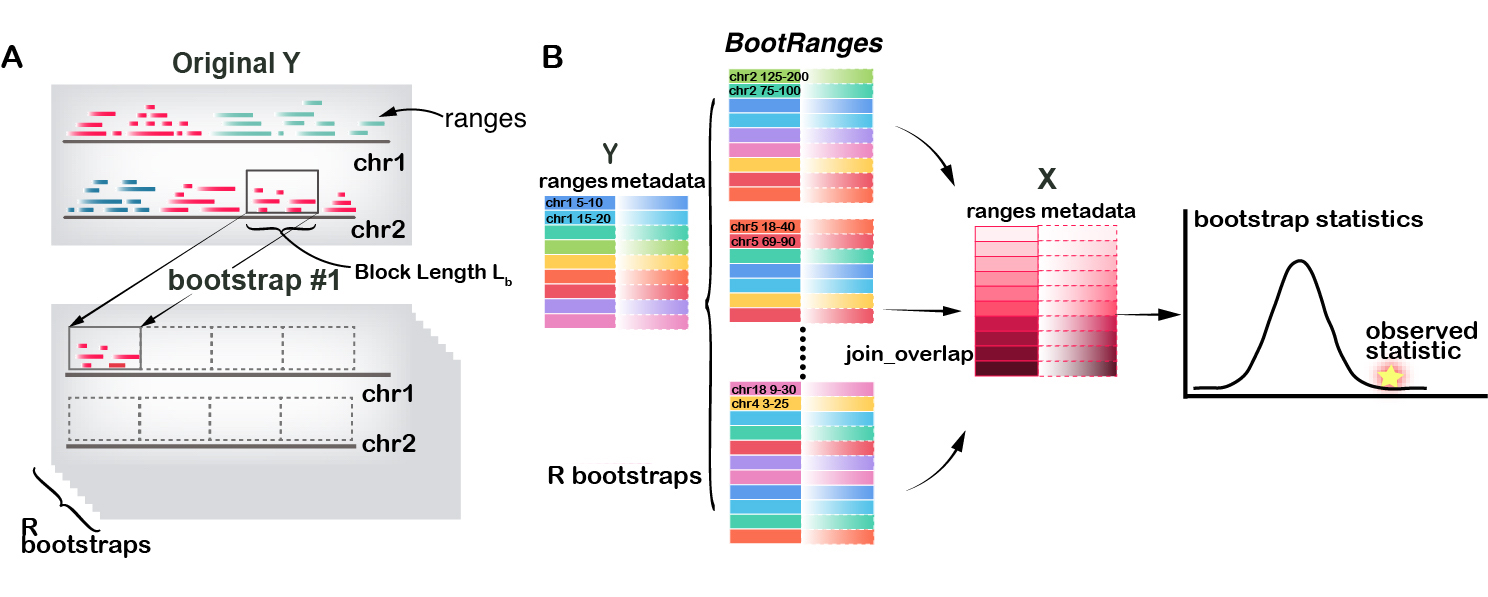
\includegraphics[scale=0.65]{Figures/bootRanges.jpg}
\caption{Overview of \bootranges workflow. (a) A schematic
  diagram of \bootranges with \texttt{blockLength} $L_b$ across chromosome.
  (b) Testing overlaps of features in \bm{$x$} with features in
  \bm{$y$}, and comparing to a null distribution.} 
\label{fig:framework}
\vspace{-0.5cm}
\end{figure}

\vspace*{-20pt}
\section{Application}

We first applied \bootranges to determine the significance of the
overlap of caQTLs detected in human liver tissue
\citep{CURRIN20211169} with SNPs associated with total cholesterol,
\mike{...where we bootstrapped the SNPs}.
While the observed overlap was significant across many combinations of
various segmentation methods and block length, the variance of the
bootstrap distribution and the resulting $z$ score varied greatly
(\cref{fig:result}A-B). Overlap rate was defined as the proportion of
SNPs within 10kb from peaks \mike{need more precise info.}
That the variance of the distribution in \cref{fig:result}A for the
unsegmented bootstrap increased with $L_b$ indicated that
bootstrapping with respect to a genome
segmentation may be a more appropriate choice
\citep{bickel2010subsampling}. 
% inhomogeneous and segmentation could alleviate the scenario.
The decreasing trend using pre-defined segmentation from
Roadmap Epigenomics indicated too many short segments,
where $L_b$ is too close to $L_s$.
\mike{maybe you can remind me how this happens}
To choose an optimal block length and segmentation, 
we considered a number of diagnostics including
those recommended previously \citep{bickel2010subsampling}:
the variance of the bootstrap distribution (\cref{fig:result}A),
a scaled version of the change in the width of the
\mike{bootstrap distribution} over $L_b$,
and the inter-feature distance distribution (Supplementary Methods).
Here $L_b \in [300\textrm{kb},600\textrm{kb}]$ was shown to be a good range for block
lengths (\cref{fig:suppfig}A-C, and Supplementary \cref{sec:results}.
The scientific conclusion of this example was that liver caQTLs were
much closer to total cholesterol SNPs than expected even when placing
blocks of SNPs to match a genome segmentation.
Simple shuffling of features (Supplementary \cref{sec:shuffle})
resulted in a much higher $z = 18.5$, compared to $z \approx 4$ for
the methods that preserve local correlation and place blocks with
respect to a genome segmentation.

%\vspace{-0.5cm}
\begin{figure}[hbtp]
\centering% default with `floatrow`
\setlength{\abovecaptionskip}{-0.1cm}
\setlength{\belowcaptionskip}{-0.1cm}
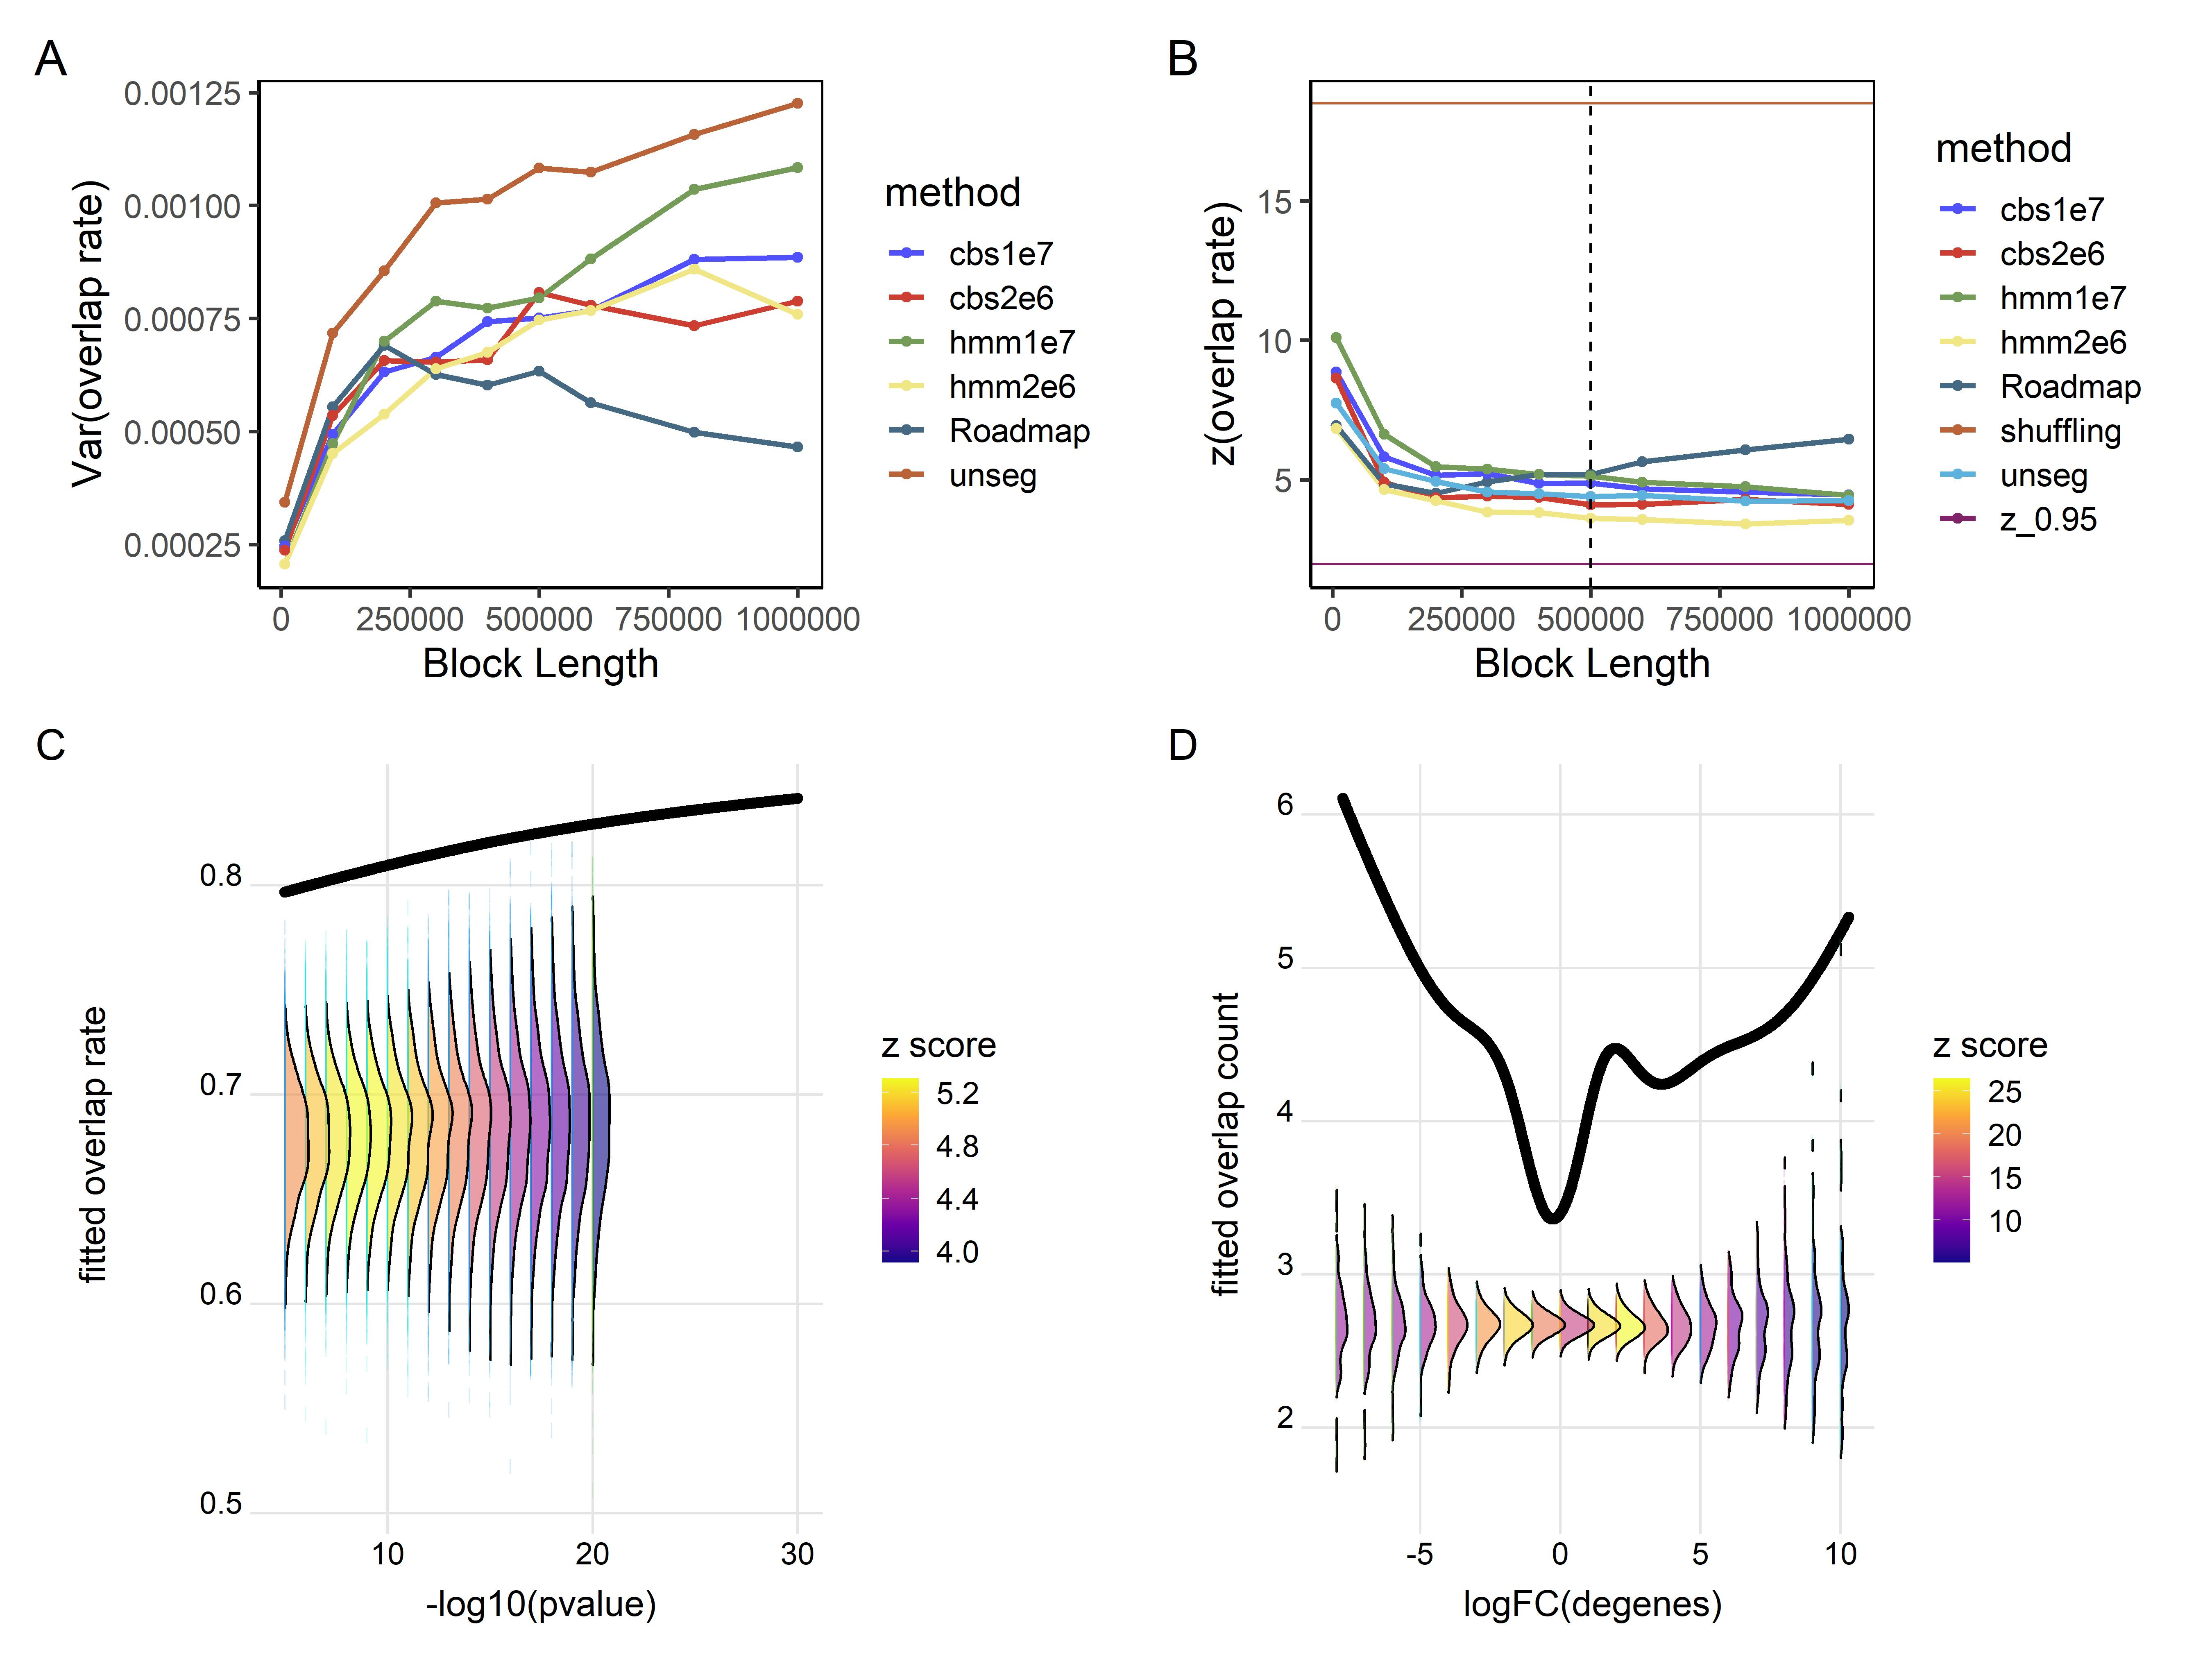
\includegraphics[scale=0.25]{Figures/fig2.jpeg}
\caption{
  Bootstrapping parameter evaluation and enrichment analyses. 
  A) Variance of the rate of overlaps and
  B) $z$ score for the observed overlap,
  for various segmentation and $L_b$ combinations on the liver caQTL
  dataset.
  %Upper and lower horizontal line represents the $z$ score obtained
  %with naive shuffling and ....
  The observed (black line) and bootstrapped (densities) overlap
  seen across various thresholds for
  C) for the overlap rate over GWAS -log10(p-value) for the liver QTL
  dataset and
  D) for the overlap count over logFC of DE genes for the macrophage
  dataset. 
  Color of density represents the $z$ score for the observed overlap
  statistic.
}
\label{fig:result}
\vspace{-0.7cm}
\end{figure}

%% z score, independent of number of bootstraps, was used to measure the
%% distance between the expected value and the observed one according to
%% the standard deviations.
%% the $z = 4.10$ if look at circular binary search(CBS)
%% \citep{cbs} segmentation method with $L_s = 2e6$ and
%% $L_b=5e5$(\cref{fig:result}B).
%% As seen in applications of \citet{bickel2010subsampling}, the effect
%% of segmentation did not greatly alter conclusions, e.g. rejection of
%% the null hypothesis, in this case, although the z score varies greatly
%% among the different segmentations and block lengths.

We demonstrate using \bootranges to motivate the choice of thresholds 
that are applied to feature sets during enrichment analyses.
We applied different thresholds to one of the feature sets, and then 
computed the observed overlap statistic and bootstrap distribution.
\mike{I have a question about how this was performed}
%In this study, we showed optimized selection of data driven p-value
%and logFC through applying \bootranges on pairs of features:
We tested this one the aforementioned liver caQTL example, to
differential chromatin accessibility and gene expression 
\citep{alasoo2018shared,lee2020fluent}.
A generalized linear model (GLM) with penalized regression splines was
fit to the observed rate or count over the -log10(p-value) or gene log
fold change (Supplementary Methods). Condition densities plotted along
with the GLM fit revealed how the threshold choice affected the
variance of the bootstrap density and the resulting $z$ score
(\cref{fig:result}C-D).
We found that the $z$ score was highest when -log10(p-value) = 8
(\cref{fig:suppfig}D),
and when the log fold change was thresholded at $< -2$ or $> 2$
(\cref{fig:suppfig}E).
%% from \textit{gam} function in the
%% \emph{mgcv} R package were fitted and \textit{predict\_gam} function
%% in the \emph{tidymv} R package were predicted on observed and each
%% null feature sets.
%% $$
%% \setlength{\abovedisplayskip}{3pt}
%% \setlength{\belowdisplayskip}{3pt}
%% log \left( \frac{\pi}{1-\pi} \right) = \beta_0  + f (-log_{10}p), log(\mu) = \beta_0 + f (log_{FC})
%% $$ 
%% for rate and count-based statistic, separately.
%% All generated 95\%
%% percentile intervals at the same time across a range of effect sizes
%% were displayed by conditional density plot 

We additionally applied \bootranges to Chromium Single Cell Multiome
ATAC + Gene Expression, to assess the correlation of the two
modalities for all pairs of genes and promoter peaks, across the 14
cell types (pseudo-bulk).  For the whole gene set, the mean
correlation of RNA-seq and ATAC log read counts was 0.33 that was
significantly far from the subsampling correlation distribution
(\cref{fig:suppfig}F) with expectation 0.007 and empirical value
indicated there was significant high correlation between genes
expression and open chromatin. Additionally, average gene-promoter
correlation per gene can be derived. XXX of genes have a significant
higher correlation.

According to the time efficiency, we compared with GSC using the
ENCODE kidney and bladder H3K27ac ChIP-seq peaks. The average time to
block bootstrap the whole genome using \bootranges is around 0.3s and
0.37s if adding the \plyranges pipeline. While GSC approximate cost
7.56s. Therefore, \bootranges is 20 times faster.
% -- maybe we can mention the code link on page 1 to save space ...
% All of the R code and data used in this paper are available at the
% following repository: 
% \url{https://github.com/Wancen/bootRangespaper}.

\vspace*{-25pt}

\section*{Funding}
This work was funded by CZI EOSS and NIH [NHGRI R01 HG009937]. 

\vspace*{-25pt}
